\documentclass{article}   	% use "amsart" instead of "article" for AMSLaTeX format
\usepackage{geometry}                		% See geometry.pdf to learn the layout options. There are lots.
\geometry{letterpaper}                   		% ... or a4paper or a5paper or ... 
\usepackage{graphicx}				% Use pdf, png, jpg, or eps§ with pdflatex; use eps in DVI mode
\usepackage{amsmath}
\usepackage{amssymb}
\usepackage{natbib}
\usepackage{lineno}
\usepackage{color}
\usepackage{hyperref}
\linenumbers


\title{DESI Observations of Type Ia Supernovae Discovered by Imaging Surveys}


\begin{document}
\maketitle

\section{DESI Reminder}
DESI is composed of two surveys.  The main Survey and the Bright Galaxy Survey (BGS) both cover 14,000 square degrees.  The
depths, exposure times, and scanning strategy differ between the two.  Both surveys are considered in this note.  The DESI surveys
run over 5 years.

\section{Host Redshifts of ZTF Discoveries with Good Light Curves}
ZTF will discover SNe~Ia that ultimately get ``good'' light curve measurements
\footnote{
\color{red} The meaning of good light curve is TBD. \color{black}}
 ZTF is expected to have discovery completeness to $z=0.15$
\color{red}
for SNe~Ia that are not significantly reddened.
\color{black}
For an imagined survey with ZTF monitoring DESI fields, Nordin has estimated the
numbers of SN~Ia discoveries, the numbers of those with good light curves, and the numbers with redshifts from the SED~Machine.
\footnote{
\color{red}
The SEDM has poor resolution so its rate of redshift success will be lower compared to other spectrographs.
\color{black}
}
The estimates are shown in Figure~\ref{ZTFnum:fig}.  (I presume some SNe with SEDM redshifts don't have good light curves.) 
The DESI footprint
is 14,000 square degrees.  
\color{red}
Assuming that the 961~SN-yr$^{-1}$  with good light curves are spatially distributed uniformly,
there will be 0.069~SN-yr$^{-1}$ per square degree, or 0.5~SN-yr$^{-1}$ per instrumented 7.5 square degree  DESI footprint.
\color{black}

\begin{figure}[h]
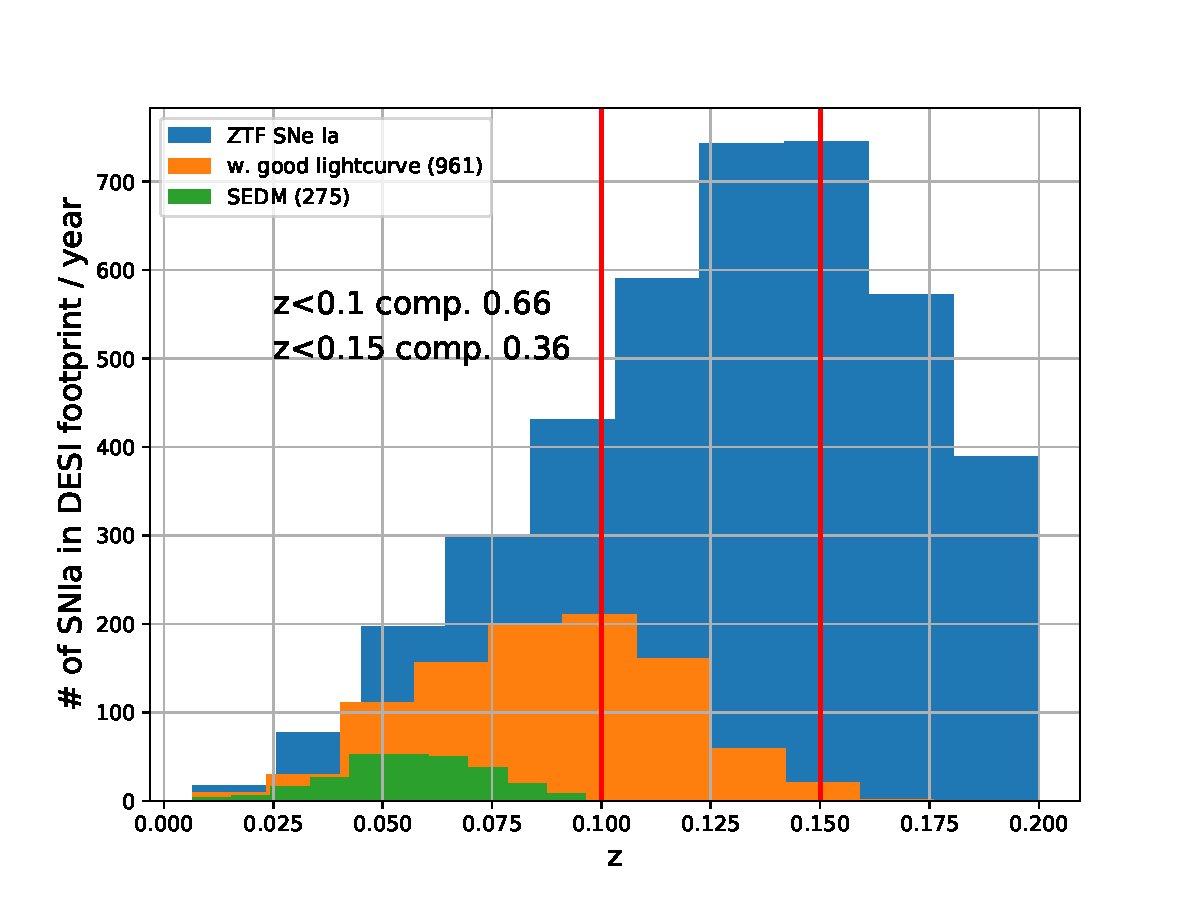
\includegraphics[width=8cm]{zdist_12m_185_195.pdf}
\centering
\caption{Numbers of ZTF SN~Ia discoveries, the numbers of those with good light curves, and the numbers with redshifts from the SED~Machine.
\label{ZTFnum:fig}}
\end{figure}

Redshifts of the host galaxies will be obtained using the SEDM, serendipitously as a DESI Bright Galaxy Survey (or other) target.
More redshifts could be obtained using spare fibers available during the DESI survey.  This note considers the latter two possibilities.

A rough estimate, described in \S\ref{details:sec},
of the fraction of supernovae in the DESI footprint
that occur in a host galaxy with a successful DESI redshift from the BGS is shown in Figure~\ref{19.5:fig}.
At redshift $z=0.15$, the upper-redshift limit for ZTF $\sim 100$\% discovery efficiency and also for objects with good light curves, half of ZTF supernovae will have a DESI redshift.
At redshift $z=0.1$, where the distribution of supernovae with good light curves peaks, 70\% of ZTF supernovae will have a DESI redshift.
That fraction increases to near-completeness as redshift decreases to zero.
The vast majority of missing redshifts come from
host galaxies that are too faint to be targeted in the BGS survey.
The remaining losses are due to
a 97 (92)\% efficiency for fiber allocation and a 92 (77)\% efficiency of extracting a redshift from the data for BGS Tier 1(2) targets. 
The deeper Survey targets
galaxies at higher redshifts than of interest for this note.

\begin{figure}[h]
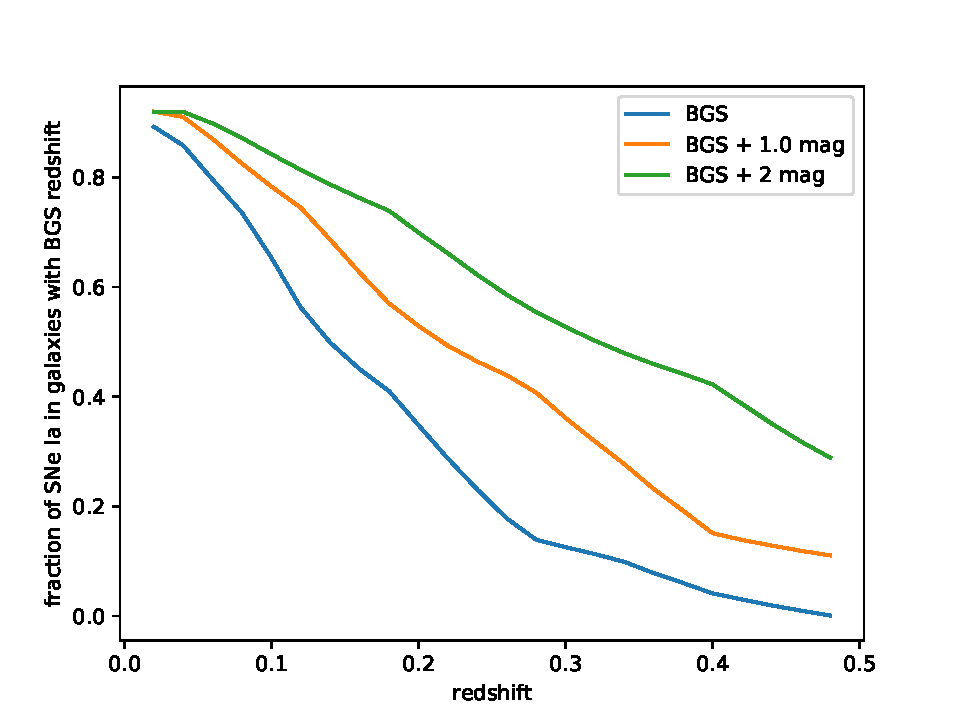
\includegraphics[width=8cm]{bg_frac.pdf}
\centering
\caption{Fraction of supernovae in the DESI footprint
that occur in a host galaxy with a successful DESI redshift from the BGS.  Also shown are  the fractions of supernovae that would occur in a host galaxy
with a successful DESI redshift (now assuming 100\% fiber-allocation efficiency) in observations 1 or 2 mag deeper than the nominal BGS exposure
(Made with  mock.py.)
\label{19.5:fig}}
\end{figure}



A candidate program to obtain redshifts of hosts not included in the BGS targets host galaxies down to a fainter magnitude limit, i.e.\ during Survey observing.
Figure~\ref{19.5:fig} shows the fractions of supernovae that would occur in a host galaxy
with a successful DESI redshift (now assuming 100\% fiber-allocation efficiency) in observations 1 or 2 mag deeper than the nominal BGS exposure.
(I believe that the standard DESI survey is 2-mag deeper than the BGS.)
This represents the fraction of supernovae in the DESI footprint
whose host could get a redshift in deeper exposures.
At redshift $z=0.15$,  $\sim 80$\% of ZTF supernovae could get a DESI redshift going 2-magnitudes deeper than BGS.
At redshift $z=0.1$, 90\% of ZTF supernovae will have a DESI redshift.


Summary: Over the course of its survey, ZTF will discover 
\color{red}
$\sim 4800$
\color{black}
SNe~Ia with good light curves.  With a matched field of view,
the DESI BGS survey will ``automatically'' obtain redshifts of a fraction of the brightest galaxies in the field, so that a significant majority
of supernovae with good light curves will have a redshift.   By targeting supernova host galaxies not in the BGS down to a fainter limiting magnitude
during the Survey,
DESI could increase the number of host-galaxy redshifts by a factor $\sim 2$ at the extreme redshift of $z=0.15$.  The number of these
extra targets would be
\color{red}
$O(1)$
\color{black}
per DESI footprint.

\section{Triggered Followup of Active Type Ia Supernovae Discovered by ZTF}
DESI can classify active SNe~Ia in its spectra, say of
a transient discovered by an imaging survey and  observed as a DESI secondary target.
For the nominal target depths of its surveys, the DESI classification efficiency curve approximates 
a unit step function with perfect classification success/failure when brighter/fainter than some $r$ limiting magnitude.  (Graur and Moustakas are recalculating these.)

To see how many objects DESI could classify in a single pointing, 
it is of interest to know how many SNe~Ia are brighter than some magnitude at any given moment.
Shown in Figure~\ref{cum:fig} are cumulative number densities of SNe~Ia that are instantaneously brighter than a limiting magnitude as a function of redshift.
Several limiting magnitudes are considered. 
As the limiting magnitude increases, the number density asymptotes at higher values and redshifts.
\color{red}
For the shallow $r_{lim}=19.5$~mag limit the density plateaus at $z \sim 0.1$ with $0.024$ objects per square degree or 0.18 per DESI footprint.   For the $r_{lim}=21.5$~mag limit the plateau occurs at $z \sim 0.3$ with $0.4$ objects per square degree or 3 per DESI footprint. 
\color{black}
The majority of transients at these magnitudes and high Galactic latitude will be SNe~Ia, so the rates for all transients would be only slightly higher.

\begin{figure}[h]
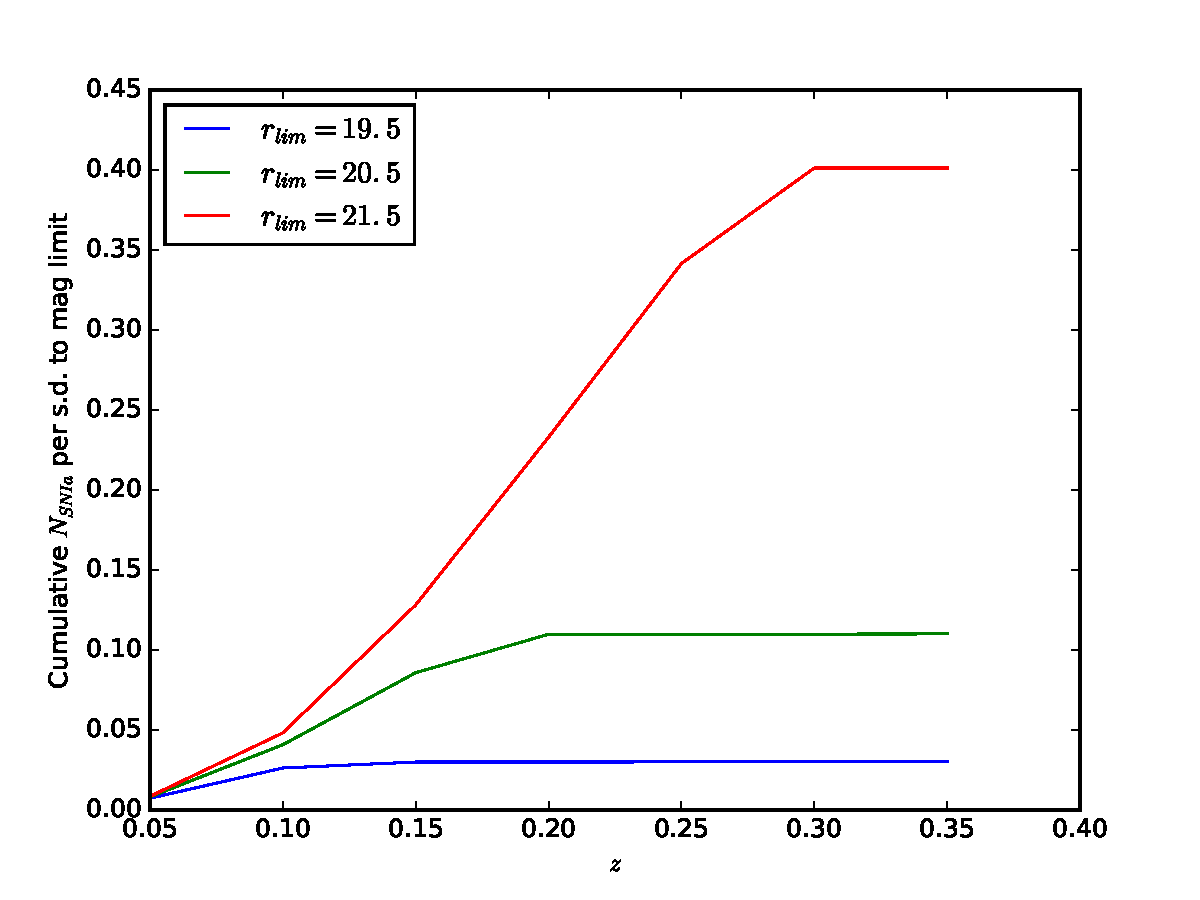
\includegraphics[width=8cm]{../src/cumulative.pdf}
\centering
\caption{Cumulative number densities as a function of redshift of SNe~Ia instantaneously brighter than several $r$ limiting magnitudes.
(Made with active.py.)
\label{cum:fig}}
\end{figure}

A ``passive'' way to trigger DESI observations of active supernovae is to request a fiber for the  transient
that happens to occur in the field DESI is pointing at.  For an imaging survey that is complete to the DESI 
$z\sim0.3$ limit, the possible transient yield is then the number of DESI pointings multiplied by the number of objects per pointing.  
\color{red}
The yield is up to 30,000 SNe~Ia for the 10,000 pointings of the
main Survey, of which 9000 would be at redshifts lower than $z<0.15$ the discovery completeness limit of ZTF.  
The yield is up to 1080 SNe~Ia for the 6000 pointings of BGS. 
\color{black}
This yield assumes that the pointings separated by time gaps gaps longer than the longest SN~Ia control time.
Most supernovae in the field, particularly those at higher redshifts, would not get a redshift.  The smaller number of supernovae at low-redshift, who have high apparent brightness
for a long time, would get a redshift.
%
%An ``active'' way to trigger DESI observations of active supernovae
%is to allocate a telescope pointing and fiber to an active transient.
%The DESI surveys get filled in stochastically following
%the random sky positions of transients.    If a transient occurs in a field that
%has already achieved its full DESI depth, it may or may not be targeted.
%To get an idea of how many pointings could potentially be actively triggered, we examine the cumulative rate of observer-frame SN~Ia explosions as a function of redshift 
%shown in Figure~\ref{total:fig}. 
%\color{red}
%To $z= 0.3$, the SN~Ia classification limit of DESI, there are $5$ SNe~Ia per square degree per year or $32$ per footprint per year.
%To $z= 0.2$, the SN~Ia discovery limit of ZTF, there are $1.2$ SNe~Ia per square degree per year or $9$ per footprint per year.  
%\color{black}
%(Recall that the discovery efficiency of ZTF drops from $z=0.15$ to 0.2.)
%\color{red}
%To $z=0.1$, the peak of the distribution of good light-curves from ZTF, there are $0.2$ SNe~Ia per square degree per year or $1.5$ per footprint per year.  
%\color{black}
%Most fields of most imaging surveys cannot be monitored for
%a full year so these numbers serve as an upper bound on the number of discovered supernovae. 
%

\color{red}
Consider ZTF as a source of active transients for DESI ``passive'' triggers when both surveys run concurrently.
ZTF discovers supernovae in fields that DESI are to observe.
As described above, each DESI Survey pointing has $O(1)$ $z<0.15$ SN~Ia targets bright enough to be classified, which adds up to
9000 classifications over all pointings.  These classified transients represent a minority of all ZTF $z<0.15$ discoveries since 
not all discoveries lie in a field DESI is about to observe.  Recall that ZTF plans to get good light curves of 4800 SNe~Ia.  Suppose
that ZTF has the flexibility to get good light curves of SNe with DESI classification.  Then a $\sim50$\% acceptance of a DESI fiber allocation is sufficient
to saturate ZTF light-curve follow-up.

The demand on the Survey can be reduced with classification with the BGS.  As described above, the BGS can passively
classify 1080 SNe~Ia.  The BGS classification rate could be increased with an
``active'' trigger, where the deterministic DESI observing schedule is perturbed to swap in fields containing
a ZTF-discovered
supernova that can be typed.
I don't think it is possible to arrange it so that every BGS pointing has a supernova; Figure~\ref{total:fig} shows that 
to $z=0.1$, the classification limit of the BGS, there are $0.2$ SNe~Ia per square degree per year or $1.5$ per footprint per year.
This caps the number of BGS classifications at 6000.  A detailed calculation is required to estimate the number of discoveries
possible with the BGS, but my intuition says that $>2000$ could be done without adding overhead to the time allocation.



%This adds up to 3750 transients over the course of 5 years.  These special transients could be prioritized for better follow-up;
%ZTF plans to get 4800
%SNe~Ia with good light curves.
%There would remain
%$\sim 1000$
%SNe with good light curves without passive DESI classification.
%These could be observed with an ``active'' trigger. 
%%Around 1000 of these triggers need to be shuffled among the 10,000 pointings.
%There should be enough ZTF discoveries  in fields not yet observed by DESI that season and so few DESI triggers,
%that no trigger observation would take time beyond that accounted for in the DESI surveys.
%Again we hope that ZTF can arrange that actively triggered supernovae also get good light curves.
\color{black}

\begin{figure}[h]
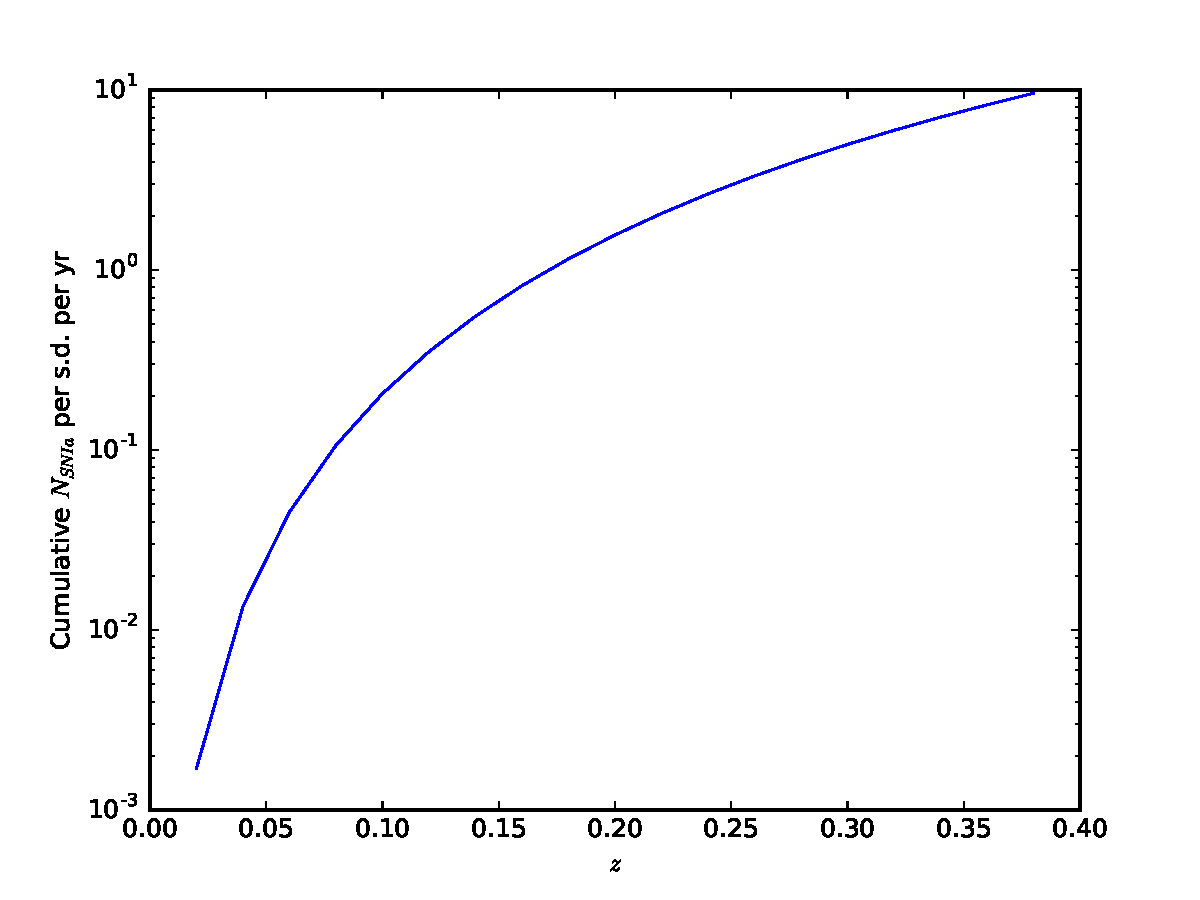
\includegraphics[width=8cm]{../src/total.pdf}
\centering
\caption{Cumulative rate of observer-frame SN~Ia explosions as a function of redshift. 
(Made with snrates.py.)
\label{total:fig}}
\end{figure}


If ZTF is not able to control which supernovae get good light curves,
DESI follow-up is still possible but there may be non-trivial
impact on the DESI survey. 
With a background active follow-up trigger, 
most of the DESI survey pointings  will not be of a triggered  and hence cover
no active ZTF-discovered transient.  However, some of those pointings
cover areas that will contain an active transient later in the season.  
A trigger could then force an observation and integration time not accounted for in the DESI Surveys.  Such observations
could be prevented but cause incompleteness in spectroscopic confirmation.
Spectroscopic resources other than DESI could fill in those gaps.
Before delving deeper into these options, let us see what kind of flexibility  ZTF has in choosing or knowing advance the
supernovae that get good light curves.

\section{Serendipitous Discovery of Active Type Ia Supernovae}
DESI can discover active SNe~Ia in the spectrum of a primary DESI target.
For now wait for properties of DESI galaxy targets and estimate rates based on those.  Figure~{cum:fig}, which shows the total number of 
supernovae in the field, shows an upper limit to the numbers of supernovae in DESI fibers.

\appendix
\section{Ugly Details}
\label{details:sec}
\color{red}
Here is what goes into the rough estimate for the fraction of supernovae with a host observed by DESI.  I use the mock BGS catalog BGS\_r20.0.hdf5.
As an  approximation of the underlying truth, I use the mock catalog 
cumulative distribution of luminosity as a function of host absolute magnitude for galaxies $0.002<z<0.004$.  Though the mock catalog misses
the  faintest galaxies, they
contribute relatively little total luminosity.
For a set of fine redshift bins, I find the absolute magnitudes that correspond to the $r=19.5$ or $20.0$ detection limit.  For each bin,
I determine how much light is in galaxies brighter than these two limits.  Assuming that the occurrence of supernovae is proportional per light, this
gives the fraction of supernovae in each bin that occur in a galaxy brighter than the limits.  There BGS survey has Tier~1 $r<19.5$ targets and Tier~2
$19.5<r<20$ targets, each with distinct fiber and redshift efficiencies.  These efficiencies are applied to each Tier, whose results are combined to give
the fraction of supernovae that occur in a galaxy with a successful DESI redshift.  This result is shown in Figure~\ref{19.5:fig}.

Jakob notes that 5\% of SNfactory supernovae ($z_{max}=0.08$) had hosts fainter than 20 mag.  Combined with the DESI targeting and redshift
efficiencies gives a  $\sim 0.8$ total efficiency, not far from the average if the redshift range shown in Figure~\ref{19.5:fig}.

\color{black}
\end{document} 
